% !TeX program = pdfLaTeX
\documentclass[smallextended]{svjour3}       % onecolumn (second format)
%\documentclass[twocolumn]{svjour3}          % twocolumn
%
\smartqed  % flush right qed marks, e.g. at end of proof
%
\usepackage{amsmath}
\usepackage{graphicx}

\usepackage[hyphens]{url} % not crucial - just used below for the URL
\usepackage{hyperref}
\providecommand{\tightlist}{%
  \setlength{\itemsep}{0pt}\setlength{\parskip}{0pt}}

%
% \usepackage{mathptmx}      % use Times fonts if available on your TeX system
%
% insert here the call for the packages your document requires
%\usepackage{latexsym}
% etc.
%
% please place your own definitions here and don't use \def but
% \newcommand{}{}
%
% Insert the name of "your journal" with
% \journalname{myjournal}
%

%% load any required packages here
\usepackage{amssymb}


\begin{document}

\title{Peaks Over Threshold for Bursty Time Series \thanks{Peter Straka was supported by the Discovery Early Career Research Award
DE160101147 on the Project ``Predicting Extremes when Events Occur in
Bursts'' by the Australian Research Council. Katharina Hees was
supported by the DAAD co-financed by the German Federal Ministry of
Education and Research (BMBF).} }



\author{  Katharina Hees \and  Smarak Nayak \and  Peter Straka* \and  }

    \authorrunning{ K. Hees, S. Nayak \& P. Straka }

\institute{
        Katharina Hees \at
     University of Dortmund \\
     \email{\href{mailto:hees@statistik.uni-dortmund.de}{\nolinkurl{hees@statistik.uni-dortmund.de}}}  %  \\
%             \emph{Present address:} of F. Author  %  if needed
    \and
        Smarak Nayak \at
     National Australia Bank \\
     \email{\href{mailto:smarak.nayak@nab.com.au}{\nolinkurl{smarak.nayak@nab.com.au}}}  %  \\
%             \emph{Present address:} of F. Author  %  if needed
    \and
        Peter Straka* \at
     UNSW Sydney \\
     \email{\href{mailto:p.straka@unsw.edu.au}{\nolinkurl{p.straka@unsw.edu.au}}}  %  \\
%             \emph{Present address:} of F. Author  %  if needed
    \and
    }

\date{Received: date / Accepted: date}
% The correct dates will be entered by the editor


\maketitle

\begin{abstract}
In many complex systems studied in statistical physics, inter-arrival
times between events such as solar flares, trades and neuron voltages
follow a heavy-tailed distribution. The set of event times is
fractal-like, being dense in some time windows and empty in others, a
phenomenon which has been dubbed ``bursty''.

This article generalizes the Peaks Over Threshold (POT) model to the
setting where inter-event times are heavy-tailed. For high thresholds
and infinite-mean waiting times, we show that the times between
threshold crossings are Mittag-Leffler distributed, and thus form a
``fractional Poisson Process'' which generalizes the standard Poisson
Process. We provide graphical means of estimating model parameters and
assessing model fit. Along the way, we apply our inference method to a
real-world bursty time series, and show how the memory of the
Mittag-Leffler distribution affects the predictive distribution for the
time until the next extreme event.
\\
\keywords{
        heavy tails \and
        renewal process \and
        extreme value theory \and
        peaks over threshold \and
    }


\end{abstract}


\def\spacingset#1{\renewcommand{\baselinestretch}%
{#1}\small\normalsize} \spacingset{1}


\section{Introduction}\label{introduction}

Time series displaying temporally inhomogeneous behaviour have received
strong interest in the recent statistical physics literature (Barabási
2005; J. Oliveira and Barabási 2005; Vasquez et al. 2006; Vazquez et al.
2007; Omi and Shinomoto 2011; Min, Goh, and Vazquez 2011; Karsai et al.
2011; Bagrow and Brockmann 2013). They have been observed in the context
of earthquakes, sunspots, neuronal activity and human communication (see
Karsai et al. 2012; Vajna, Tóth, and Kertész 2013; Mark M Meerschaert
and Stoev 2008 for a list of references). Such time series exhibit high
activity in some `bursty' intervals, which alternate with other, quiet
intervals. Although several mechanisms are plausible explanations for
bursty behaviour (most prominently self-exciting point process by Hawkes
(1971)), there seems to be one salient feature which very typically
indicates the departure from temporal homogeneity: a heavy-tailed
distribution of waiting times (Vasquez et al. 2006; Karsai et al. 2012;
Vajna, Tóth, and Kertész 2013). As we show below in simulations, a
simple renewal process with heavy-tailed waiting times can capture this
type of dynamics. For many systems, the renewal property is appropriate;
a simple test of the absence of correlations in a succession of waiting
times can be undertaken by randomly reshuffling the waiting times
(Karsai et al. 2012).

Often a magnitude, or mark can be assigned to each event in the renewal
process, such as for earthquakes, solar flares or neuron voltages. The
Peaks-Over-Threshold model (POT, see e.g. Coles 2001) applies a
threshold to the magnitudes, and fits a Generalized Pareto distribution
to the threshold exceedances. A commonly made assumption in POT models
is that times between events are either fixed or light-tailed, and this
entails that the threshold crossing times form a Poisson process (Hsing,
Hüsler, and Leadbetter 1988). Then as one increases the threshold and
thus decreases the threshold crossing probability \(p\), the Poisson
process is rarefied, i.e.~its intensity decreases \emph{linearly} with
\(p\) (see e.g. Beirlant et al. 2006).

As will be shown below, in the heavy-tailed waiting time scenario
threshold crossing times form a \emph{fractional Poisson process}
(Laskin 2003; Mark M Meerschaert, Nane, and Vellaisamy 2011), which is a
renewal process with Mittag-Leffler distributed waiting times. The
family of Mittag-Leffler distributions nests the exponential
distribution (Haubold, Mathai, and Saxena 2011), and hence the
fractional Poisson process generalizes the standard Poisson process.
Again as the threshold size increases and the threshold crossing
probability \(p\) decreases, the fractional Poisson process is rarefied:
The scale parameter of the Mittag-Leffler inter-arrival times of
threshold crossing times increases, but \emph{superlinearly}; see the
Theorem below.

Maxima of events which occur according to a renewal process with
heavy-tailed waiting times have been studied under the names
``Continuous Time Random Maxima process'' (CTRM) (Benson, Schumer, and
Meerschaert 2007; Mark M Meerschaert and Stoev 2008; Hees and Scheffler
2016; Hees and Scheffler 2017), ``Max-Renewal process'' (Silvestrov
2002; Silvestrov and Teugels 2004; Basrak and Špoljarić 2015), and
``Shock process'' (Esary and Marshall 1973; Shanthikumar and Sumita
1983; Shanthikumar and Sumita 1984; Shanthikumar and Sumita 1985;
Anderson 1987; Gut and Hüsler 1999). The existing literature focuses on
probabilistic results surrounding these models. In this work, however,
we introduce a method of inference for this type of model, which is
seemingly not available in the literature.

We review the marked renewal process in Section 2, and derive a scaling
limit theorem for inter-exceedance times in Section 3. We give a
statistical procedure to estimate model parameters via stability plots
in Section 5, but to set the stage we first discuss inference for the
Mittag-Leffler distribution in Section 4. (A simulation study of the
effectiveness of our statistical procedure is given in the appendix.)
Diagnostic plots for model criticism are discussed in Section 6. In
Section 7, we discuss the memory property of the Mittag-Leffler
distribution, and how it affects the predictive distribution for the
time until the next threshold crossing event. Section 8 concludes. For
all statistical computations we have used R (R Core Team 2018). All code
and data used for the analysis in this article has been organized into
an R package \texttt{CTRE} (\url{https://github.com/UNSW-MATH/CTRE}).
The source code for the figures generated in this manuscript is
available online at \url{https://github.com/UNSW-MATH/bursty-POT}.

\section{Continuous Time Random Exceedances
(CTRE)}\label{continuous-time-random-exceedances-ctre}

As a model for extreme observations, we use a Marked Renewal Process
(MRP):

\begin{description}
\item[\textbf{Definition (MRP):}]
Let \((W,J), (W_1, J_1), (W_2, J_2), \ldots\) be i.i.d. pairs of random
variables, where the \(W_k > 0\) are interpreted as the \emph{waiting
times} and \(J_k \in [x_L, x_R]\) as the \emph{event magnitudes}
(\(x_L \in [-\infty, +\infty), x_R \in (-\infty, +\infty]\)). If \(W\)
and \(J\) are independent, the Marked Renewal Process is said to be
\emph{uncoupled}. \qed
\end{description}

Note that the \(k\)-th magnitude \(J_k\) occurs at time
\(T_k = W_1 + \ldots + W_k\). Based on an MRP, we define the Continuous
Time Random Exceedance model (CTRE) as follows:

\begin{description}
\item[\textbf{Definition (CTRE):}]
Given a threshold \(\ell \in (x_L, x_R)\), consider the stopping time
\[\tau(\ell) := \min\{k: J_k > \ell\},\quad \ell \in (x_L, x_R).\]
Define the pair of random variables \((X(\ell), T(\ell))\) via
\[X(\ell) = J_{\tau(\ell)} - \ell, \quad 
T(\ell) = \sum_{k=1}^{\tau(\ell)} W_k.\] By restarting the MRP at
\(\tau(\ell)\), inductively define the two i.i.d. sequences
\(T(\ell,n)\) and \(X(\ell, n)\), \(n \in \mathbb N\), called the
``interarrival times'' and the ``exceedances'', respectively. The pair
sequence \((T(\ell, n), W(\ell, n))_{n \in \mathbb N}\) is called a
Continuous Time Random Exceedance model (CTRE). If the underlying MRP is
uncoupled, then the CTRE is also called uncoupled. \qed
\end{description}

\begin{figure}
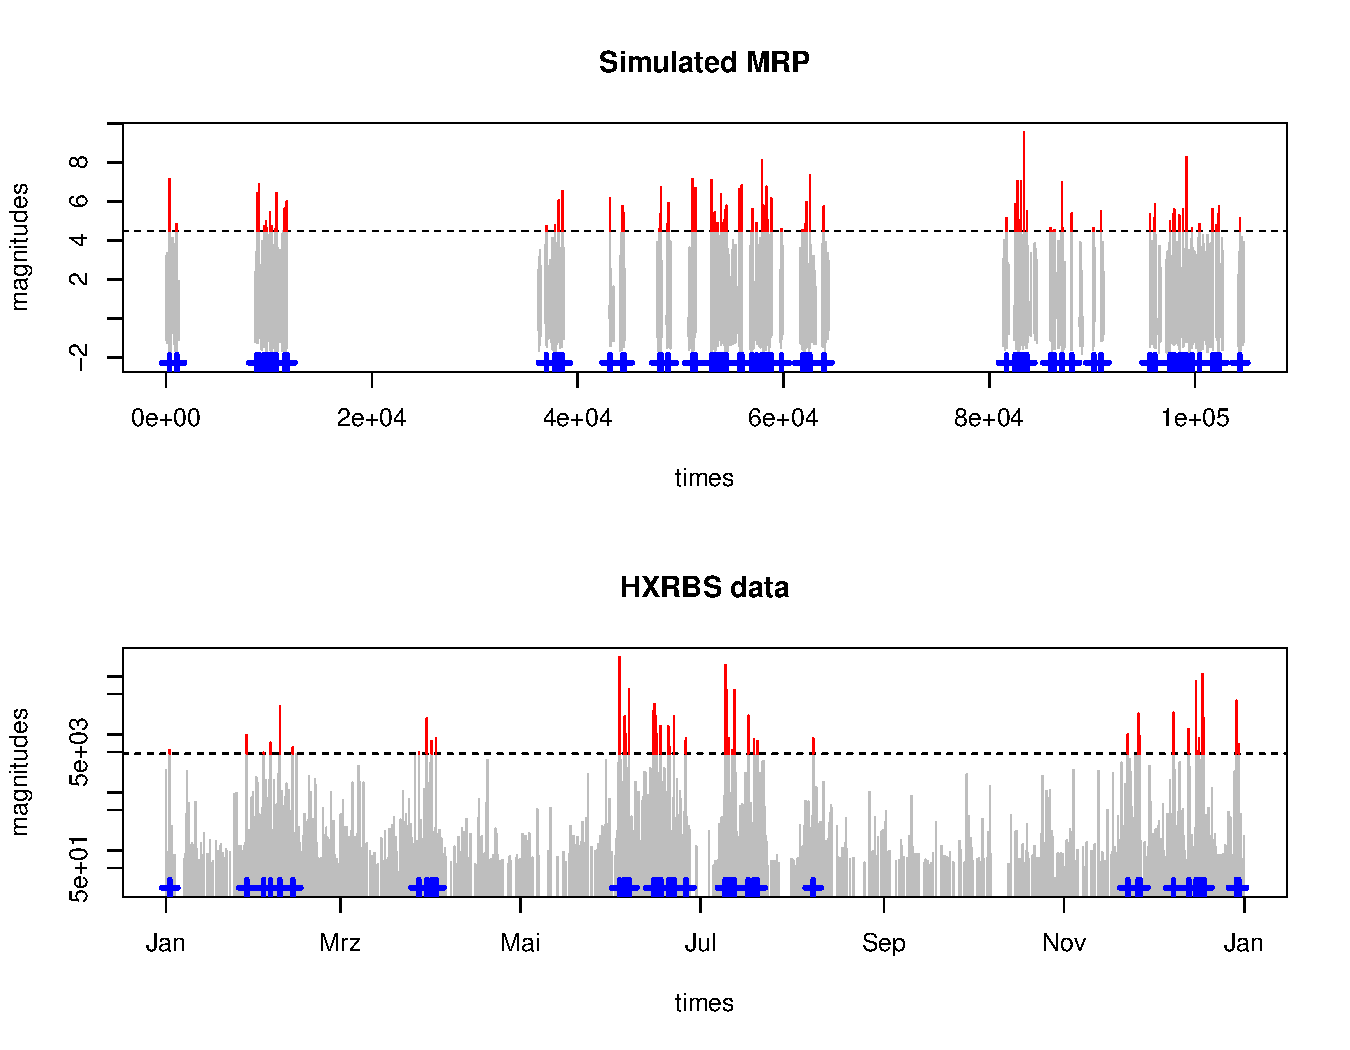
\includegraphics[width=\textwidth]{article_springer_files/figure-latex/thresholdedBursty-1} \caption{\label{fig:thresholdedBursty}Exceedances (red) and Times until Exceedance (durations between blue crosses) for a given threshold $\ell$ (dashed line).}\label{fig:thresholdedBursty}
\end{figure}

In this article, we restrict ourselves to the uncoupled case, where the
two sequences \(X(\ell, n)_{n \in \mathbb N}\) and
\(T(\ell, n)_{n \in \mathbb N}\) are independent.\footnote{To see why,
  note that \(X(\ell)\) is, in distribution, simply equal to
  \(J | J > \ell\), independent of any waiting time \(W_k\).} Figure
\ref{fig:thresholdedBursty} shows a simulated dataset in the top panel,
where \(W\) has a stable distribution with tail parameter \(\beta =\)
0.8 (and skewness \(1\) and location \(0\)), and where \(J\) is from a
standard Gumbel distribution. In the bottom panel, we plot a time series
of solar flare intensities derived from a NASA dataset (Dennis et al.
1991)\footnote{The ``complete Hard X Ray Burst Spectrometer event list''
  is a comprehensive reference for all measurements of the Hard X Ray
  Burst Spectrometer on NASA's Solar Maximum Mission from the time of
  launch on Feb 14, 1980 to the end of the mission in Dec 1989. 12,776
  events were detected, with the ``vast majority being solar flares''.
  The list includes the start time, peak time, duration, and peak rate
  of each event. We have used ``start time'' as the variable for event
  times, and ``peak rate'' as the variable for event magnitudes.}.
Clearly, the simulated data exhibit long intervals \emph{without any}
events, whereas in the real-world dataset events appear continuously.
The threshold exceedances, however, appear to have similar statistical
behaviour in both models. Observations below a threshold are commonly
discarded in Extreme Value Theory (POT approach); likewise, the CTRE
model interprets these observations as noise and filters them out.

\section{Scaling limit of Exceedance Times}\label{sec:scaling}

In this section we state and prove the key theorem, see below. For an
accessible introduction to regular variation and stable limit theorems,
we recommend the book by Mark M Meerschaert and Sikorskii (2012).

\begin{description}
\tightlist
\item[\textbf{Theorem:}]
Let the waiting times \(J_k\) be in the domain of attraction of a
positively skewed sum-stable law with stability parameter
\(0 < \beta < 1\); more precisely,

\begin{align} \label{eq:stability}
\frac{W_1 + \ldots + W_n}{b(n)} \overset{d}{\longrightarrow} D, 
\quad n \to \infty
\end{align}

for a function \(b(n)\) which is regularly varying at \(\infty\) with
parameter \(1/\beta\), and where
\(\mathbf E[\exp(-sD)] = \exp(-s^\beta)\). Write
\(p := \mathbf P(J > \ell)\). Then the weak convergence \[
\frac{T(\ell)} {b(1/p)} \to W_\beta \quad \text{ as } \quad \ell \uparrow x_R
\] holds, where the Mittag-Leffler random variable \(W_\beta\) is
defined on the positive real numbers via \[
\mathbf E[\exp(-sW_\beta)] = \frac{1}{1+s^\beta}.
\] \qed
\end{description}

\noindent For a scale parameter \(\sigma > 0\), we write
\({\rm ML}(\beta, \sigma)\) for the distribution of \(\sigma W_\beta\).
The Mittag-Leffler distribution with parameter \(\beta \in (0,1]\) is a
heavy-tailed positive distribution for \(\beta < 1\), with infinite
mean. However, as \(\beta \uparrow 1\), \({\rm ML}(\beta, \sigma)\)
converges weakly to the exponential distribution \({\rm Exp}(\sigma)\).
This means that although its moments are all infinite, the
Mittag-Leffler distribution may (if \(\beta\) is close to 1) be
indistinguishable from the exponential distribution, for the purposes of
applied statistics. For a detailed reference on the Mittag-Leffler
distribution, see e.g. Haubold, Mathai, and Saxena (2011), and for
algorithms, see e.g.~the R package \texttt{MittagLeffleR} (Gill and
Straka 2017).

\paragraph{\texorpdfstring{\emph{Proof of
Theorem:}}{Proof of Theorem:}}\label{proof-of-theorem}

We interpret the threshold crossing time \(T(\ell)\) as the hitting time
of the underlying CTRM (Continuous Time Random Maxima) or ``max-renewal
process'', and then utilize a result by Mark M Meerschaert and Stoev
(2008). The running maximum process is defined as \[
M(c) := J_1 \vee \ldots \vee J_{\lfloor c \rfloor},
\] and since we assume that the \(J_k\) have a continuous distribution,
there exist norming functions \(a(c)\) and \(d(c)\) such that \[
\mathbf P\left[ \frac{M(c) - d(c)}{a(c)} \le \ell^* \right] 
\longrightarrow F(\ell^*), \quad t \to \infty
\] where \(F\) is a generalized extreme value distribution, and
\(\ell^*\) is any value from the support of \(F\). The CTRM process is
then defined via \[
V(t) = M(N(t)), \quad t \ge 0
\] where \(N(t)\) is the renewal process associated with the waiting
times \(W_k\): \[
N(t) = \max\{n: W_1 + \ldots + W_n \le t\}.
\] Now a key observation is that \[
T(\ell) = \inf\{t: V(t) > \ell\}, 
\] and that \[
T(\ell) > t \quad \text{ if and only if } \quad V(t) \le \ell.
\] By (Theorem 3.1, Mark M Meerschaert and Stoev 2008), we have the
stochastic process convergence \[
\frac{V(ct) - d(\tilde b(c))}{a(\tilde b(c))} 
\stackrel{d}{\longrightarrow} Y(t), \quad t > 0.
\] where \(Y(t)\) is a time-changed (``subordinated'') extremal process,
and where \(\tilde b(c)\) is a regularly varying norming function which
is \emph{inverse} to \(b(c)\), in the sense that
\(b(\tilde b(c)) \sim c \sim \tilde b(b(c))\).

Without loss of generality, we choose \(\ell^*\) such that
\(F(\ell^*) = 1/e\), and let
\(\ell = a(\tilde b(c)) \ell^* + d(\tilde b(c))\). We may then calculate
\[
\mathbf P\left[ \frac{T(\ell)}{b(1/p)} > t \right]
= \mathbf P[T(\ell) > b(1/p) t]
= \mathbf P[V(ct) \le \ell]
\] where we have substituted \(c = b(1/p)\). Moreover \[
\mathbf P[V(ct) \le \ell]
= \mathbf P\left[ \frac{V(ct) - d(\tilde b(c))}{a(\tilde b(c))} 
\le \frac{\ell - d(\tilde b(c))}{a(\tilde b(c))} \right]
\longrightarrow \mathbf P\left[ Y(t) \le \ell^* \right]
\] Defining the hitting time of level \(\ell^*\) by \(Y(t)\) as
\(\xi_{\ell^*} := \inf\{t: Y(t) > \ell^*\}\), we then have \[
P\left[ Y(t) \le \ell^* \right] = \mathbf P[\xi_{\ell^*} > t] 
= \mathbf P[(-\log F(\ell^*))^{-1/\beta} X^{1/\beta} D > t]
\] by (Proposition 4.2, Mark M Meerschaert and Stoev 2008), where \(X\)
is an exponential random variable with mean \(1\). Using (Theorem 19.1,
Haubold, Mathai, and Saxena 2011), we see that
\(X^{1/\beta} D \sim {\rm ML}(\beta, 1)\), concluding the proof. \qed

\begin{description}
\tightlist
\item[\textbf{Remark:}]
If \(\beta = 1\), the result of the Theorem above is standard, see e.g.
Equation (2.2) in Gut and Hüsler (1999).
\end{description}

\section{Inference for the Mittag-Leffler
distribution}\label{inference-for-the-mittag-leffler-distribution}

\begin{figure}
\includegraphics[width=\textwidth]{article_springer_files/figure-latex/fig:QQ-plots-1} \caption{Pareto vs. Mittag-Leffler distribution, both with same tail exponent 0.8. Top row: solar flare magnitudes data, fitting nicely with a Pareto distribution. Bottom row: simulated Mittag-Leffler data. Left column: static QQ-Estimator plots, assessing a fit against the Pareto distribution. Centre column: dynamic QQ-Estimator plots. Right column: a usual QQ-Plot based on Mittag-Leffler quantiles.\label{fig:QQ-plots}}\label{fig:fig:QQ-plots}
\end{figure}

Since the Mittag-Leffler distribution is heavy-tailed, many researchers
would intuitively give the highest importance to the tail behaviour of
the distribution, and estimate the exponent of the tail function with
established methods such as the Hill estimator. The QQ-estimator (Kratz
and Resnick 1996) is closely related to the Hill estimator and fits a
least squares line through the logarithms of the ordered statistics
(y-axis) and the corresponding quantiles of the exponential distribution
(x-axis). The reciprocal slope is returned as the estimate of the tail
exponent. For instance, the top-left panel in Figure \ref{fig:QQ-plots}
shows the (static) QQ-estimator for the magnitudes of the solar flare
data, returning a good fit to a Pareto distribution with tail parameter
0.79. The dynamic QQ-estimator plot (top-center panel) plots the tail
exponent estimate for the largest values at cutoffs varying up to the
5th order statistic, and the region of stability at 0.8 indicates a
recommended estimate.

However, as described nicely by Resnick (1997), the less similar a
heavy-tailed distribution is to a Pareto distribution, the less useful a
Hill or QQ-Plot estimator becomes. The bottom-left panel of Figure
\ref{fig:QQ-plots}, for instance, shows the static QQ-estimator plot for
\(2000\) draws from the Mittag-Leffler distribution with tail parameter
\(0.8\). The stretched exponential shape means that the Mittag-Leffler
distribution has more probability near \(0\) than the Pareto
distribution, severely biasing the estimator downwards (0.67). Even by
looking at different cutoffs via the dynamic QQ-estimator plot
(bottom-center panel) one hardly identifies \(0.8\) as a clear candidate
for a tail parameter estimate.

QQ-estimators, and the closely related Hill estimator, are hence not
suitable to detect a heavy-tailed Mittag-Leffler distribution. Moreover,
QQ-estimator plots of exponentially distributed data are virtually
indistinguishable from the bottom-left panel. This shows that
\emph{Mittag-Leffler distributed data may look like exponentially
distributed data if examined via a QQ-estimator}.

Hence if there is some prior expectation that the data are drawn from
the Mittag-Leffler distribution (as is the the case for threshold
exceedance times), then we recommend avoiding QQ-estimators and Hill
plots altogether, and instead examining QQ-plots directly, on a
logarithmic scale (see Figure \ref{fig:QQ-plots}, right column). The
scale parameter \(\sigma\) is irrelevant for a QQ-Plot. The tail
parameter \(\beta\) can be estimated quickly via the log-moment method
by Cahoy (2013), or via maximum likelihood. Both estimators are
implemented in \texttt{MittagLeffleR} (Gill and Straka 2017). Since the
exponential distribution is nested in the Mittag-Leffler family of
distributions, a standard likelihood ratio test can be performed, with
the exponential distribution as a null model against a Mittag-Leffler
distribution as the alternative. As an example, the threshold crossing
times for the solar flare dataset (Figure \ref{fig:flare-diagnostics-2},
right panel) yield a difference in deviance of \(\approx\) 324, which
evaluates to a strongly significant \(\chi^2_1\) test statistic (p-value
= \(10^{-72}\)) for the null hypothesis \(\beta = 1\).

\section{Inference on Exceedance
times}\label{inference-on-exceedance-times}

\begin{figure}
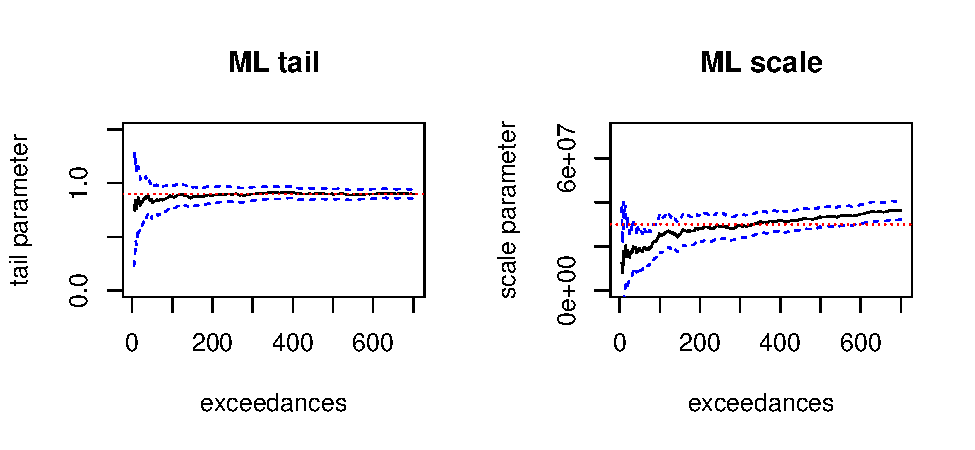
\includegraphics[width=\textwidth]{article_springer_files/figure-latex/solar-flare-tail-scale-1} \caption{\label{fig:flares}Stability plots for the tail and scale parameter of the Mittag-Leffler distribution of the Solar Flare dataset. Dotted horizontal lines are at $\beta = 0.85$ and $\sigma_0 = 3 \times 10^7$ seconds $\approx 0.95$ years.}\label{fig:solar-flare-tail-scale}
\end{figure}

The Theorem in Section \ref{sec:scaling} implies that for a high
threshold \(\ell\) we may approximate the distribution of \(T(\ell)\)
with an \({\rm ML}(\beta, b(1/p))\) distribution, where \(b(\,)\) varies
regularly at \(\infty\) with parameter \(1/\beta\). Building on the POT
(Peaks Over Threshold) method, we propose the following estimation
procedure for the distribution of \(T(\ell)\):

\begin{enumerate}
\def\labelenumi{\arabic{enumi}.}
\item
  For a range of thresholds \(\ell\) near the largest order statistics,
  extract datasets of exceedance times \(\{T(\ell, i)\}_i\).
\item
  For each choice of threshold \(\ell\), fit a Mittag-Leffler
  distribution to the resulting dataset \(\{T(\ell, i)\}_i\). This
  results in the estimates \(\{\hat\beta(\ell)\}_\ell\) and
  \(\{\hat \sigma(\ell)\}_\ell\).
\item
  Plot \(\ell\) vs.~\(\hat \beta(\ell)\). As \(\ell\) increases towards
  \(x_R\), \(\hat \beta(\ell)\) \emph{stabilizes} around a constant
  \(\hat \beta\). Use \(\hat \beta\) as an estimate for the tail
  parameter \(\beta\) of the Mittag-Leffler distribution of exceedance
  times.
\item
  Approximate \(p \approx |\{k: J_k > \ell\}| / n\). Recall that
  \(b(c)\) is regularly varying with parameter \(1/\beta\), and hence
  has the representation \(b(c) = L(c) c^{1/\beta}\) for some slowly
  varying function \(L(c)\). Assuming that the variation of \(L(c)\) is
  negligible, we hence plot \(\ell\)
  vs.~\(p^{1/\hat \beta} \hat \sigma(\ell)\). Again as \(\ell\)
  increases towards \(x_R\), \(p^{1/\hat \beta} \hat \sigma(\ell)\) is
  expected to stabilize around a constant \(\hat \sigma_0\). We then use
  \(p^{-1/\hat \beta} \hat \sigma_0\) as an estimate of the scale
  parameter of the Mittag-Leffler distribution of exceedance times for
  the level \(\ell\).
\end{enumerate}

The above approach, though theoretically sound, benefits from the
following practical adjustments (compare with Figure \ref{fig:flares}):

\begin{itemize}
\tightlist
\item
  We choose \(\ell\) from the order statistics, i.e. \(\ell\) is the
  \(k\)-th largest of the observations \(X_j\), where \(k\) runs from
  \(k_\text{min}, k_\text{min} + 1, \ldots, k_\text{max}\). The datasets
  are then of length \(k-1\).
\item
  We use \(k\) rather than \(\ell\) for the horizontal axis of our
  plots.
\item
  In Step 4, rather than plotting \(p^{1/\hat \beta} \hat \sigma(\ell)\)
  we plot \(k^{1/\hat \beta} \hat \sigma(\ell)\). This changes
  \(\hat \sigma_0\) by the multiplicative constant \(n^{1/\hat \beta}\),
  but has the advantage that \(\hat \sigma_0\) does not change if one
  pre-processes the data by removing all observations below a certain
  threshold.
\end{itemize}

The estimates \(\hat \beta\) and \(\hat \sigma_0\) give an estimate of
the distribution of exceedance times, dependent on the threshold
\(\ell\):

\begin{align*}
T(\ell) \sim {\rm ML}(\hat \beta, k^{-1/\hat \beta} \hat \sigma_0).
\end{align*}

For quick estimates of the Mittag-Leffler parameters we have used the
method of log-transformed moments by Cahoy (2013). We have verified the
validity of our estimation algorithm via simulations, see the appendix.

\section{Checking Model Assumptions}\label{checking-model-assumptions}

\begin{figure}
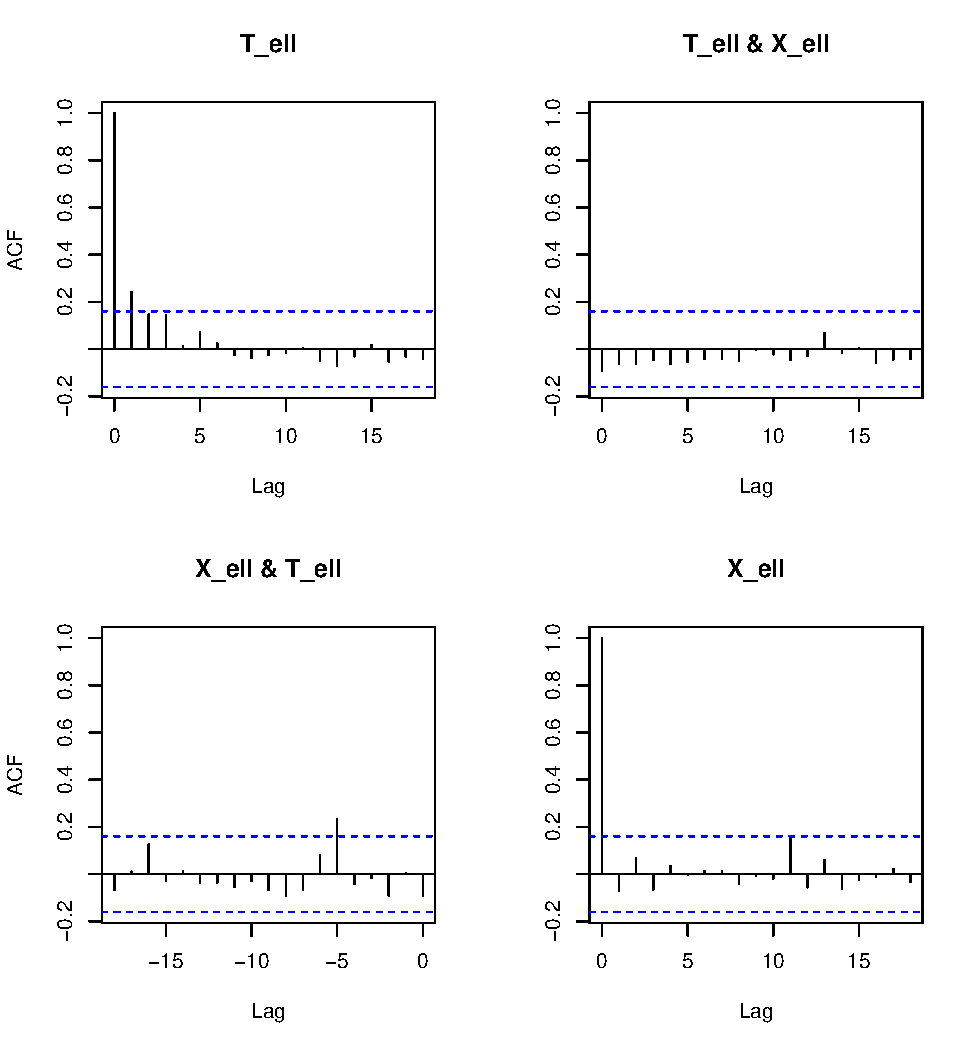
\includegraphics[width=\textwidth]{article_springer_files/figure-latex/flare-diagnostics-1-1} \caption{Diagnostic plots for the solar flare data: auto-correlation function.\label{fig:flare-diagnostics-1}}\label{fig:flare-diagnostics-1}
\end{figure}

\begin{figure}
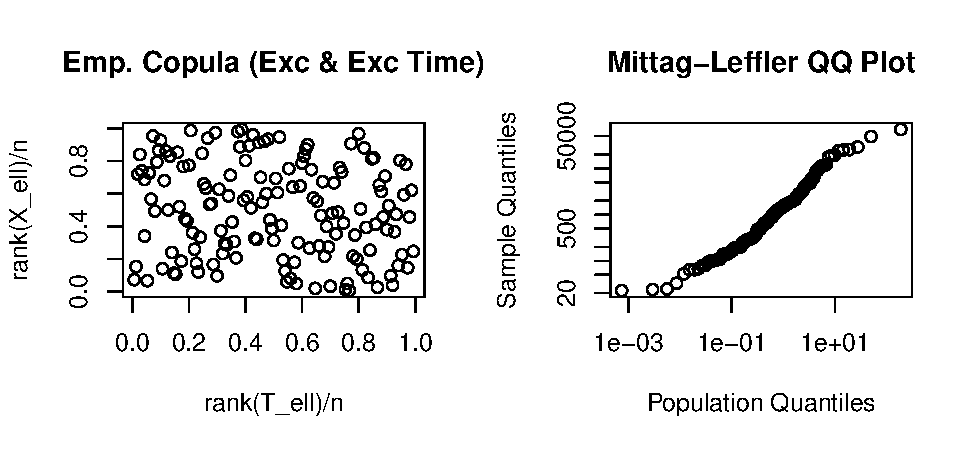
\includegraphics[width=\textwidth]{article_springer_files/figure-latex/flare-diagnostics-2-1} \caption{Diagnostic plots for the solar flare data: empirical copula and QQ Plot. \label{fig:flare-diagnostics-2}}\label{fig:flare-diagnostics-2}
\end{figure}

The CTRE model is based on three main assumptions, which are repeated
below. For each assumption, we suggest one means of checking if it
holds:

\begin{description}
\tightlist
\item[i.i.d.:]
After removing the ``noise observations'' below the smallest threshold
\(\ell_0\), the pair sequence \((T(\ell_0, i), X(\ell_0,i))\) is i.i.d.
An indication if this is true is given by an auto-correlation plot for
the logarithms (to ensure finite moments) of the two time series.
\item[Uncoupled:]
Each \(T(\ell, i)\) is independent of each \(X(\ell, i)\). We propose an
empirical copula plot to check for any dependence.
\item[\({\rm ML}(\beta, \sigma)\) distribution of \(T(\ell, i)\):]
Apply a cutoff at the lowest threshold \(\ell_0\), extract the threshold
crossing times, and create a QQ Plot for the Mittag-Leffler
distribution. Use a log-Moment estimate of the tail parameter for the
theoretical / population quantiles of the plot.
\end{description}

Figures \ref{fig:flare-diagnostics-1} and \ref{fig:flare-diagnostics-2}
show the diagnostic plots for a minimum threshold chosen at the 200th
order statistic. There is some residual autocorrelation for the sequence
of threshold exceedance times that is not accounted for by the CTRE
model. The fit with a Mittag-Leffler distribution (\(\beta = 0.8\)) is
good, though there are signs that the power-law tail tapers off for very
large inter-threshold crossing times. There is no apparent dependence
between threshold exceedance times and event magnitudes seen in the
copula plot.

\section{Predicting the time of the next threshold
crossing}\label{predicting-the-time-of-the-next-threshold-crossing}

According to Figure \ref{fig:flares}, for a threshold \(\ell\) at the
\(k\)-th order statistic, the fitted threshold exceedance time
distribution is \[
T_\ell \sim {\rm ML}(\beta, k^{1/\beta} \sigma_0), 
\] where \(\beta = 0.85\) and \(\sigma_0 = 3.0 \times 10^7 {\rm sec}\).
Unlike the exponential distribution, the Mittag-Leffler distribution is
not memoryless, and the probability density of the time \(t\) until the
next threshold crossing will depend on the time \(t_0\) elapsed since
the last threshold crossing. This density equals \[
p(t|\beta, \sigma_0, \ell, t_0) = \frac{f(t + t_0 | \beta, k^{1/\beta} \sigma_0)}{\mathbf P[T_\ell > t_0]}
\] where \(f(\,\cdot\, | \beta, k^{1/\beta} \sigma_0)\) is the
probability density of \({\rm ML}(\beta, k^{1/\beta} \sigma_0)\). The
more time has passed without a threshold crossing, the more the
probability distribution shifts towards larger values for the next
crossing (see Figure \ref{fig:hazard}, left panel). The hazard rate \[
h(t) = \frac{f(t| \beta, k^{1/\beta} \sigma_0))}{\int_t^\infty f(\tau| \beta, k^{1/\beta} \sigma_0))\,d\tau}
\] represents the risk of a threshold crossing per unit time, and is a
decreasing function for the Mittag-Leffler distribution. The closer
\(\beta\) is to \(1\), the more the hazard rate mimics that of an
exponential distribution (a constant function, see Figure
\ref{fig:hazard}, right panel).

\begin{figure}
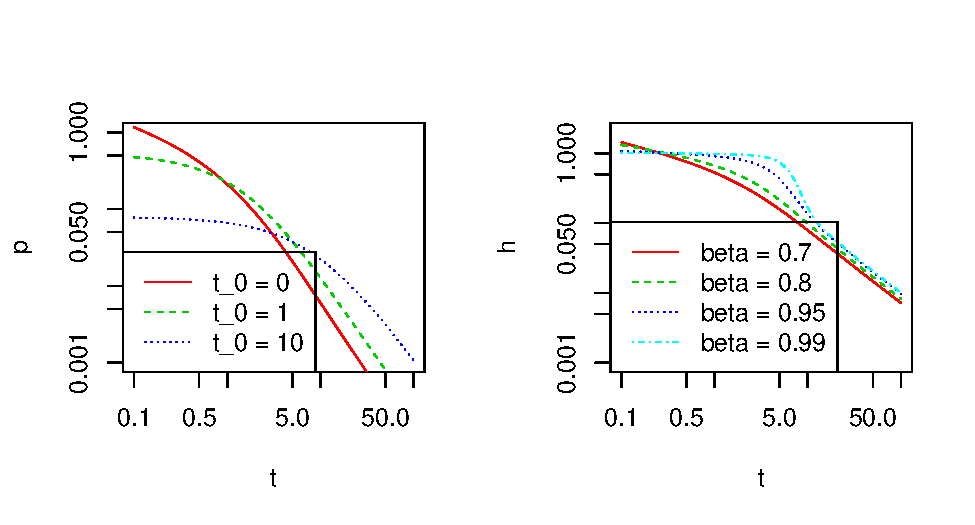
\includegraphics[width=\textwidth]{article_springer_files/figure-latex/hazard-1} \caption{Left: Conditional distribution of time until next threshold crossing, depending on elapsed time $t_0$ since last crossing ($\beta = 0.8$, $\sigma_0 = 1$). Right: Hazard rate depending on tail parameter $\beta$.\label{fig:hazard}}\label{fig:hazard}
\end{figure}

It is beyond the scope of the current paper to incorporate parameter
uncertainty into our predictive distribution for the next threshold
crossing; however, methods as described by Scarrott and Macdonald (2012)
and Lee, Fan, and Sisson (2015) are likely to extend to our setting.

\section{Discussion \& Conclusion}\label{discussion-conclusion}

We have extended the POT (Peaks over Threshold) model, a mainstay of
extreme value theory, to ``bursty'' time series, which have been studied
intensively in statistical physics. Burstiness is characterized by
power-law waiting times between events, and we have shown that the
Mittag-Leffler distribution arises naturally as a scaling limit for the
inter-exceedance times of high thresholds. Moreover, we have derived the
following non-linear scaling behaviour: \(\sigma \sim p^{-1/\beta}\),
where \(\sigma\) is the scale parameter of the distribution of threshold
exceedance times, \(p\) is the fraction of magnitudes above the
threshold, and \(\beta\) the exponent of the power law. This
``anomalous'' scaling behaviour in the bursty setting entails two
phenomena: i) a heavy tail of the interarrival time distribution of
threshold crossings (long rests), and ii) a high propensity for more
threshold crossing events immediately after each threshold crossing
event (bursts). The Mittag-Leffler distribution captures both phenomena,
due to its heavy tail as well as its stretched exponential (peaked)
asymptotics for small times. It generalizes the exponential
distribution, and in the solar flare data example, this generalization
is warranted, because the likelihood-ratio test is strongly significant.

When we introduced the CTRE model, we assumed that all events are i.i.d.
This assumption is likely sufficient but not necessary for our limit
theorem to hold. Moreover, any data below a (minimum) threshold
\(\ell_0\) is discarded for CTREs, and hence need not satisfy the i.i.d.
assumption. For the purposes of statistical inference, we merely require
that the inter-threshold-crossing times are i.i.d.

The bursty CTRE approach to model ``non-Poissonian'' threshold crossing
times should be contrasted with the (now standard) approach of clusters
of extremes, see e.g. Ferro and Segers (2003). In this approach, i.i.d.
event sequences of magnitudes are generalized to stationary sequences of
event magnitudes (subject to a mixing condition). The two approaches are
fundamentally different: A clustering model assumes that each event
belongs to one particular (latent) group of events. For bursts, however,
the aim is to identify an underlying scale-free pattern in the event
dynamics, which is often characteristic of complex systems. It is an
interesting open problem to develop quality criteria, based e.g.~on
measures of surprise (Lee, Fan, and Sisson 2015), which guide an applied
statistician in the choice between a clustering and a CTRE approach for
a particular problem. Moreover, we believe it may be possible to unify
the two approaches by considering CTREs based on MRPs with a
\emph{stationary}, rather than i.i.d., sequence of magnitudes.

Finally, a purely scale-free pattern for event times may be too rigid an
assumption for some bursty time series, because often the heavy-tailed
character of the inter-arrival time distribution does not hold at all
time scales; rather, it applies at short and intermediate time scales,
and is truncated (or tempered, reverting to an exponential distribution)
at very long time scales (see e.g. Mark M. Meerschaert, Roy, and Shao
2012; and Aban, Meerschaert, and Panorska 2006). In such situations, a
``tempered'' Mittag-Leffler distribution may provide a more realistic
fit, which we aim to introduce in follow-up work.

\subsection*{Acknowledgements}\label{acknowledgements}
\addcontentsline{toc}{subsection}{Acknowledgements}

The authors would like to thank Prof.~Peter Scheffler for insights on
stochastic process limits for CTRMs, and Gurtek Gill who helped create
the MittagLeffleR R-package.
\newpage 

\section*{Appendix}

\appendix

\section{Validating our inference method on simulated
data}\label{validating-our-inference-method-on-simulated-data}

To test our inference method via stability plots, we have simulated
10000 independent waiting time and magnitude pairs \((W_k, J_k)\) (see
upper panel in Figure \ref{fig:thresholdedBursty}). In order to have
exact analytical values available for \(\beta\) and \(\sigma_0\), a
distribution for \(W_k\) needs to be chosen for which \(b(n)\) from
\eqref{eq:stability} is known. If we choose \(W_k \stackrel{d}{=} D\),
where \(D\) is as in \eqref{eq:stability}, then due to the stability
property we have the \emph{equality} of distribution
\(W_1 + \ldots + W_n \stackrel{d}{=} b(n) D\), for
\(b(n) = n^{1/\beta}\). Using the parametrisation of Samorodnitsky and
Taqqu (1994), a few lines of calculation (see e.g.~the vignette on
parametrisation in Gill and Straka (2017)) show that \(D\) must have the
stable distribution \(S_\beta(\cos(\pi \beta/2)^{1/\beta}, +1, 0)\),
which is implemented in the R package \texttt{stabledist} by Wuertz,
Maechler, and members. (2016).

\begin{figure}[b]
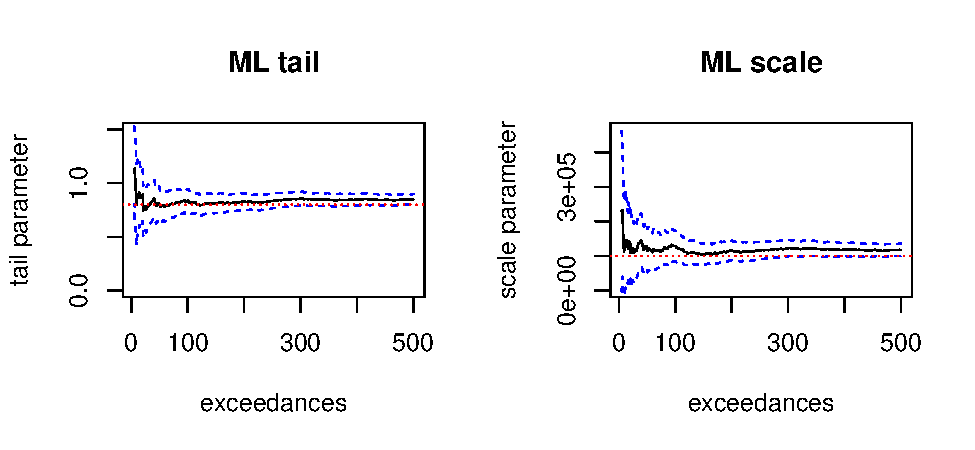
\includegraphics[width=\textwidth]{article_springer_files/figure-latex/simulated-example-1} \caption{Tail and scale estimates for simulated data, with waiting times drawn from the stable distribution $S_\beta(\cos(\pi \beta/2)^{1/\beta}, +1, 0)$ with $\beta = 0.8$. Dashed lines are 95\% confidence intervals, dotted lines are the known theoretical values ($0.8$ and $10000^{1/0.8}$). \label{fig:sim}}\label{fig:simulated-example}
\end{figure}

By the Theorem, the distribution of \(T(\ell)\) is approximately \[
{\rm ML}(\beta, p^{-1/\beta}) 
= {\rm ML}(\beta, k^{-1/\beta} n^{1/\beta}),
\] which means \(\sigma_0 = n^{1/\beta}\). The distribution of \(J_k\)
is irrelevant for the inference on \(\beta\) and \(\sigma_0\) (we have
chosen unit exponential random variables). Figure \ref{fig:sim} displays
plots of \(\hat \beta(\ell)\) and \(\hat \sigma(\ell)\) vs. \(k\);
recall that \(k\) is the index of the order statistics of \(J_k\) at
which the threshold \(\ell\) is placed. Dotted lines show 95\%
confidence intervals, which are derived from the asymptotic normality of
the log-moments estimators (Cahoy 2013) and the \(\delta\)-method (Gill
and Straka 2017). The dashed lines show the actual values of \(\beta\)
resp.~\(\sigma_0\), showing that our inference method identifies the
parameters correctly.

%\section*{References}\label{references}
%\addcontentsline{toc}{section}{References}
\bibliography{CTRMstats}
\bibliographystyle{spbasic}


\hypertarget{refs}{}
\hypertarget{ref-Aban06}{}
Aban, Inmaculada B, Mark M Meerschaert, and Anna K Panorska. 2006.
``Parameter Estimation for the Truncated Pareto Distribution.'' \emph{J.
Am. Stat. Assoc.} 101 (473): 270--77.
doi:\href{https://doi.org/10.1198/016214505000000411}{10.1198/016214505000000411}.

\hypertarget{ref-Anderson1987}{}
Anderson, Kevin K. 1987. ``Limit Theorems for General Shock Models with
Infinite Mean Intershock Times.'' \emph{J. Appl. Probab.} 24 (2):
449--56. \url{http://www.jstor.org/stable/3214268}.

\hypertarget{ref-Bagrow2013}{}
Bagrow, James P., and Dirk Brockmann. 2013. ``Natural emergence of
clusters and bursts in network evolution.'' \emph{Phys. Rev. X} 3 (2):
1--6.
doi:\href{https://doi.org/10.1103/PhysRevX.3.021016}{10.1103/PhysRevX.3.021016}.

\hypertarget{ref-Barabasi2005}{}
Barabási, Albert László. 2005. ``The origin of bursts and heavy tails in
human dynamics.'' \emph{Nature} 435 (May): 207--11.
doi:\href{https://doi.org/10.1038/nature03459}{10.1038/nature03459}.

\hypertarget{ref-Basrak2014}{}
Basrak, Bojan, and Drago Špoljarić. 2015. ``Extremes of random variables
observed in renewal times.'' \emph{Stat. Probab. Lett.} 97. Elsevier
B.V.: 216--21.
doi:\href{https://doi.org/10.1016/j.spl.2014.11.025}{10.1016/j.spl.2014.11.025}.

\hypertarget{ref-beirlantBook}{}
Beirlant, Jan, Yuri Goegebeur, Johan Segers, and Jozef Teugels. 2006.
\emph{Statistics of extremes: theory and applications}. John Wiley \&
Sons.

\hypertarget{ref-Benson2007}{}
Benson, David A, Rina Schumer, and Mark M Meerschaert. 2007.
``Recurrence of extreme events with power-law interarrival times.''
\emph{Geophys. Res. Lett.} 34 (l16404): DOI:10.1029/2007GL030767.
doi:\href{https://doi.org/10.1029/2007GL030767}{10.1029/2007GL030767}.

\hypertarget{ref-Cahoy2013}{}
Cahoy, Dexter O. 2013. ``Estimation of Mittag-Leffler Parameters.''
\emph{Commun. Stat. - Simul. Comput.} 42 (2): 303--15.
doi:\href{https://doi.org/10.1080/03610918.2011.640094}{10.1080/03610918.2011.640094}.

\hypertarget{ref-ColesBook}{}
Coles, S. 2001. \emph{An Introduction to Statistical Modelling of
Extreme Values}. London: Springer-Verlag.

\hypertarget{ref-HXRBS}{}
Dennis, Brian R, L E Orwig, G S Kennard, G J Labow, R A Schwartz, A R
Shaver, and A K Tolbert. 1991. ``The complete Hard X Ray Burst
Spectrometer event list, 1980-1989.''
\url{https://umbra.nascom.nasa.gov/smm/hxrbs.html}.

\hypertarget{ref-Esary1973}{}
Esary, J. D., and A. W. Marshall. 1973. ``Shock Models and Wear
Processes.''
doi:\href{https://doi.org/10.1214/aop/1176996891}{10.1214/aop/1176996891}.

\hypertarget{ref-ferro2003inference}{}
Ferro, Christopher AT, and Johan Segers. 2003. ``Inference for Clusters
of Extreme Values.'' \emph{Journal of the Royal Statistical Society:
Series B (Statistical Methodology)} 65 (2). Wiley Online Library:
545--56.

\hypertarget{ref-MittagLeffleR}{}
Gill, Gurtek, and Peter Straka. 2017. \emph{MittagLeffleR: Using the
Mittag-Leffler Distributions in R}.
\url{https://strakaps.github.io/MittagLeffleR/}.

\hypertarget{ref-Gut1999}{}
Gut, Allan, and Jürg Hüsler. 1999. ``Extreme Shock Models.''
\emph{Extremes}, no. 1983: 295--307.
\url{http://link.springer.com/article/10.1023/A:1009959004020}.

\hypertarget{ref-Haubold11}{}
Haubold, H.J., A. M. Mathai, and R. K. Saxena. 2011. ``Mittag-Leffler
Functions and Their Applications.'' \emph{J. Appl. Math.} 2011: 1--51.
doi:\href{https://doi.org/10.1155/2011/298628}{10.1155/2011/298628}.

\hypertarget{ref-hawkes1971point}{}
Hawkes, Alan G. 1971. ``Point spectra of some mutually exciting point
processes.'' \emph{J. R. Stat. Soc. Ser. B Stat. Methodol.} JSTOR,
438--43.

\hypertarget{ref-Hees16}{}
Hees, Katharina, and Hans-Peter Scheffler. 2016. ``On joint sum/max
stability and sum/max domains of attraction,'' June, 1--31.
\url{http://arxiv.org/abs/1606.03109}.

\hypertarget{ref-Hees17}{}
---------. 2017. ``Coupled Continuous Time Random Maxima.''
\emph{Extremes}, no. June (September). Extremes: 1--24.
doi:\href{https://doi.org/10.1007/s10687-017-0304-6}{10.1007/s10687-017-0304-6}.

\hypertarget{ref-Hsing88}{}
Hsing, T, J Hüsler, and M R Leadbetter. 1988. ``On the Exceedance Point
Process for a Stationary Sequence'' 78: 97--112.

\hypertarget{ref-Karsai2012}{}
Karsai, Márton, Kimmo Kaski, Albert László Barabási, and János Kertész.
2012. ``Universal features of correlated bursty behaviour.'' \emph{Sci.
Rep.} 2.
doi:\href{https://doi.org/10.1038/srep00397}{10.1038/srep00397}.

\hypertarget{ref-Karsai2011}{}
Karsai, Márton, M. Kivelä, R. K. Pan, K. Kaski, J. Kertész, Albert
László Barabási, and J. Saramäki. 2011. ``Small but slow world: How
network topology and burstiness slow down spreading.'' \emph{Phys. Rev.
E - Stat. Nonlinear, Soft Matter Phys.} 83: 1--4.
doi:\href{https://doi.org/10.1103/PhysRevE.83.025102}{10.1103/PhysRevE.83.025102}.

\hypertarget{ref-Kratz96}{}
Kratz, Marie, and Sidney I. Resnick. 1996. ``The qq-estimator and heavy
tails.'' \emph{Commun. Stat. Part C Stoch. Model.} 12 (4): 699--724.
doi:\href{https://doi.org/10.1080/15326349608807407}{10.1080/15326349608807407}.

\hypertarget{ref-Laskin2003}{}
Laskin, Nick. 2003. ``Fractional Poisson process.'' \emph{Commun.
Nonlinear Sci. Numer. Simul.} 8 (3-4): 201--13.
doi:\href{https://doi.org/10.1016/S1007-5704(03)00037-6}{10.1016/S1007-5704(03)00037-6}.

\hypertarget{ref-Lee15}{}
Lee, J., Y. Fan, and S. A. Sisson. 2015. ``Bayesian threshold selection
for extremal models using measures of surprise.'' \emph{Comput. Stat.
Data Anal.} 85. Elsevier B.V.: 84--99.
doi:\href{https://doi.org/10.1016/j.csda.2014.12.004}{10.1016/j.csda.2014.12.004}.

\hypertarget{ref-MeerschaertSikorskii}{}
Meerschaert, Mark M, and Alla Sikorskii. 2012. \emph{Stochastic Models
for Fractional Calculus}. Vol. 43. Walter de Gruyter.

\pagebreak

\hypertarget{ref-MeerschaertStoev08}{}
Meerschaert, Mark M, and Stilian A Stoev. 2008. ``Extremal limit
theorems for observations separated by random power law waiting times.''
\emph{J. Stat. Plan. Inference} 139 (7): 2175--88.
doi:\href{https://doi.org/10.1016/j.jspi.2008.10.005}{10.1016/j.jspi.2008.10.005}.

\hypertarget{ref-Meerschaert2010b}{}
Meerschaert, Mark M, Erkan Nane, and P. Vellaisamy. 2011. ``The
fractional Poisson process and the inverse stable subordinator.''
\emph{Electron. J. Probab.} 16: 1600--1620.
doi:\href{https://doi.org/10.1214/EJP.v16-920}{10.1214/EJP.v16-920}.

\hypertarget{ref-MeerschaertRoyQin}{}
Meerschaert, Mark M., Parthanil Roy, and Qin Shao. 2012. ``Parameter
estimation for exponentially tempered power law distributions.''
\emph{Commun. Stat. - Theory Methods} 41 (10): 1839--56.
doi:\href{https://doi.org/10.1080/03610926.2011.552828}{10.1080/03610926.2011.552828}.

\hypertarget{ref-Min2010}{}
Min, Byungjoon, K. I. Goh, and Alexei Vazquez. 2011. ``Spreading
dynamics following bursty human activity patterns.'' \emph{Phys. Rev. E
- Stat. Nonlinear, Soft Matter Phys.} 83 (3): 2--5.
doi:\href{https://doi.org/10.1103/PhysRevE.83.036102}{10.1103/PhysRevE.83.036102}.

\hypertarget{ref-Oliveira2005}{}
Oliveira, J, and Albert László Barabási. 2005. ``Darwin and Einstein
correspondence patterns.'' \emph{Nature} 437 (October): 1251.
doi:\href{https://doi.org/10.0138/4371251a}{10.0138/4371251a}.

\hypertarget{ref-Omi2011}{}
Omi, Takahiro, and Shigeru Shinomoto. 2011. ``Optimizing Time Histograms
for Non-Poissonian Spike Trains.'' \emph{Neural Comput.} 23 (12):
3125--44.
doi:\href{https://doi.org/10.1162/NECO_a_00213}{10.1162/NECO\_a\_00213}.

\hypertarget{ref-R}{}
R Core Team. 2018. \emph{R: A Language and Environment for Statistical
Computing}. Vienna, Austria: R Foundation for Statistical Computing.
\url{https://www.R-project.org/}.

\hypertarget{ref-Resnick97}{}
Resnick, Sidney I. 1997. ``Heavy tail modeling and teletraffic data.''
\emph{Ann. Stat.} 25 (5): 1805--49.
doi:\href{https://doi.org/10.1214/aos/1069362376}{10.1214/aos/1069362376}.

\hypertarget{ref-SamorodnitskyTaqqu}{}
Samorodnitsky, Gennady, and Murad S Taqqu. 1994. \emph{Stable
Non-Gaussian Random Processes: Stochastic Models with Infinite
Variance}. Stochastic Modeling. London: Chapman Hall.

\hypertarget{ref-Scarrott12}{}
Scarrott, Carl, and Anna Macdonald. 2012. ``A REVIEW OF EXTREME VALUE
THRESHOLD ESTIMATION AND UNCERTAINTY QUANTIFICATION.'' \emph{REVSTAT --
Stat. J.} 10 (1): 33--60.

\hypertarget{ref-Sumita1983}{}
Shanthikumar, J. George, and Ushio Sumita. 1983. ``General shock models
associated with correlated renewal sequences.'' \emph{J. Appl. Probab.}
20 (3): 600--614. \url{http://www.jstor.org/stable/3213896}.

\hypertarget{ref-Sumita1984}{}
---------. 1984. ``Distribution Properties of the System Failure Time in
a General Shock Model.'' \emph{Adv. Appl. Probab.} 16 (2): 363--77.
\url{http://www.jstor.org/stable/1427074}.

\hypertarget{ref-Sumita1985}{}
---------. 1985. ``A class of correlated cumulative shock models.''
\emph{Adv. Appl. Probab.} 17 (2): 347--66.
\url{http://www.jstor.org/stable/1427145}.

\hypertarget{ref-Silvestrov2002a}{}
Silvestrov, Dmitrii S. 2002. \emph{Limit Theorems for Randomly Stopped
Stochastic Processes}. Springer (Berlin, Heidelberg).

\hypertarget{ref-ST04}{}
Silvestrov, Dmitrii S, and Jozef L. Teugels. 2004. ``Limit theorems for
mixed max-sum processes with renewal stopping.'' \emph{Ann. Appl.
Probab.} 14 (4): 1838--68.
doi:\href{https://doi.org/10.1214/105051604000000215}{10.1214/105051604000000215}.

\hypertarget{ref-Vajna2013}{}
Vajna, Szabolcs, Bálint Tóth, and János Kertész. 2013. ``Modelling
bursty time series.'' \emph{New J. Phys.} 15 (10): 103023.
doi:\href{https://doi.org/10.1088/1367-2630/15/10/103023}{10.1088/1367-2630/15/10/103023}.


\hypertarget{ref-Vasquez2006}{}
Vasquez, a, J G Oliveira, Z Dezso, K-I Goh, I Kondor, and Albert László
Barabási. 2006. ``Modeling bursts and heavy tails in human dynamics.''
\emph{Phys. Rev. E} 73: 361271--3612718.

\hypertarget{ref-Vazquez2007}{}
Vazquez, Alexei, Balázs Rácz, András Lukács, and Albert László Barabási.
2007. ``Impact of non-poissonian activity patterns on spreading
processes.'' \emph{Phys. Rev. Lett.} 98 (APRIL): 1--4.
doi:\href{https://doi.org/10.1103/PhysRevLett.98.158702}{10.1103/PhysRevLett.98.158702}.

\hypertarget{ref-stabledist}{}
Wuertz, Diethelm, Martin Maechler, and Rmetrics core team members. 2016.
\emph{Stabledist: Stable Distribution Functions}.
\url{https://CRAN.R-project.org/package=stabledist}.



\end{document}
